\documentclass[10pt,a4paper]{article}

\usepackage[margin=1.45cm]{geometry}
\usepackage{graphicx}
\usepackage{subcaption}
\usepackage{booktabs}
\usepackage{multirow}
\usepackage{amsmath,amssymb}
\usepackage{hyperref}
\usepackage[french]{babel}

\setlength{\parindent}{0pt}
\setlength{\parskip}{2pt}
\setlength{\textfloatsep}{6pt}
\setlength{\floatsep}{5pt}
\setlength{\intextsep}{5pt}
\setlength{\abovecaptionskip}{3pt}
\setlength{\belowcaptionskip}{0pt}

\newcommand{\R}{\mathbb{R}}

\title{\vspace{-1.2cm}Prédiction multi-label de genres de films à partir de posters\\[0.05em]
\small Hi! PARIS -- Challenge B2Ideas}
\author{Alexandre Schulz}

\begin{document}

\maketitle

\section{Introduction}
Le challenge consiste à prédire les genres d'un film à partir de son poster. Il s'agit d'un problème de classification multi-label : un même film peut appartenir à plusieurs genres. Dans ce rapport, nous présentons une méthodologie basée sur le fine-tuning de modèles pré-entraînés de la littérature : ResNet~\cite{he2016}, CLIP~\cite{radford2021} et DeiT~\cite{touvron2021}. 

Un poster contient différents indices visuels utiles pour cette tâche : palette de couleurs, composition, typographie, présence de personnages ou d'objets caractéristiques, ainsi que du texte directement visible sur l'image.

\paragraph{Les données.}
Le dataset est composé de posters de films associés à un ou plusieurs genres parmi 19 classes.
Il s'agit donc d'un problème de classification multi-label, contrairement à une classification multi-classe classique.
La distribution des genres est déséquilibrée, ce qui motive l'utilisation d'une binary cross-entropy pondérée pendant l'entraînement et de métriques comme le macro-F1 et la mAP pour l'évaluation.

\section{Choix de modélisation et entraînement} 
Nous comparons trois modèles pré-entraînés : ResNet-50, DeiT-Small et CLIP ViT-B/32.
Pour chaque modèle, la tête de prédiction est remplacée par un MLP composé de deux couches cachées de dimension 512, avec activation GELU et dropout de 0.5, suivi d'une couche linéaire finale produisant 19 logits, un par genre.
Les logits sont optimisés avec une binary cross-entropy pondérée, adaptée au cadre multi-label et au déséquilibre des classes.

L'entraînement est effectué en deux étapes.
Dans un premier temps, seul le classifieur final est entraîné afin d'adapter les représentations pré-entraînées au dataset.
Dans un second temps, l'ensemble du modèle est fine-tuné avec un learning rate plus faible.
Pour chaque modèle, nous conservons le meilleur checkpoint selon la mAP de validation, puis nous l'évaluons sur le jeu de test.

\section{Évaluation et résultats}

Le code, les configurations et les scripts d'évaluation sont disponibles sur GitHub.\footnote{\url{https://github.com/Dolgalad/HiParis_B2Ideas_challenge}. Le README contient des analyses complémentaires, des figures additionnelles et les instructions de reproduction. Expériences réalisées sur GPU NVIDIA A40.}

\paragraph{Métriques.}
Les modèles produisent une probabilité $\hat p_k(x)$ pour chaque genre $k$.
Pour les scores F1, les prédictions sont binarisées avec un seuil $\tau=0.5$.
Pour chaque genre, on définit
\[
F1_k = \frac{2TP_k}{2TP_k + FP_k + FN_k}.
\]
Le macro-F1 est la moyenne non pondérée des $F1_k$ sur les genres, ce qui donne la même importance aux classes rares et fréquentes.
Le micro-F1 agrège d'abord les $TP$, $FP$ et $FN$ sur tous les genres avant de calculer le F1, et reflète donc davantage la performance globale.
Enfin, la mAP est calculée à partir des scores continus, sans seuillage, en moyennant l'average precision obtenue pour chaque genre.

\begin{table}[htbp]
\centering
\resizebox{\linewidth}{!}{
\begin{tabular}{lcccccccc}
\multirow{2}{*}{\textbf{Modèle}}
& \multicolumn{4}{c}{\textbf{Étape 1}}
& \multicolumn{4}{c}{\textbf{Étape 2}} \\
\cmidrule(lr){2-5} \cmidrule(lr){6-9}
& Epoch & Micro-F1 $\uparrow$ & Macro-F1 $\uparrow$ & mAP $\uparrow$
& Epoch & Micro-F1 $\uparrow$ & Macro-F1 $\uparrow$ & mAP $\uparrow$ \\
\midrule
ResNet-50 & $30$ & $0.4602$          & $0.3129$          & $0.3065$          & $49$ & $0.4778$          & $0.3443$          & $0.3466$ \\
CLIP ViT-B/32   & $23$ & $\mathbf{0.5626}$ & $\mathbf{0.4104}$ & $\mathbf{0.4171}$ & $45$ & $\mathbf{0.5747}$ & $\mathbf{0.4167}$ & $\mathbf{0.4353}$ \\
DeiT-Small   & $18$ & $0.5021$          & $0.3838$          & $0.3870$          & $37$ & $0.5106$          & $0.3830$          & $0.3804$ \\
\bottomrule
\end{tabular}}
\caption{Comparaison des performances sur le jeu de test selon les étapes d'entraînement.}
\label{tab:stage-results}
\end{table}

Les résultats de la Table~\ref{tab:stage-results} montrent que CLIP obtient les meilleures performances, avec un micro-F1 de $0.5747$, un macro-F1 de $0.4167$ et une mAP de $0.4353$ après fine-tuning.
Cette supériorité est cohérente avec son pré-entraînement image-texte, particulièrement adapté aux posters de films qui combinent des indices visuels, typographiques et sémantiques.
ResNet bénéficie également du fine-tuning, tandis que DeiT progresse peu après la première étape, ce qui suggère une adaptation moins efficace au dataset ou un risque de sur-apprentissage.

\begin{figure}[htbp]
\centering
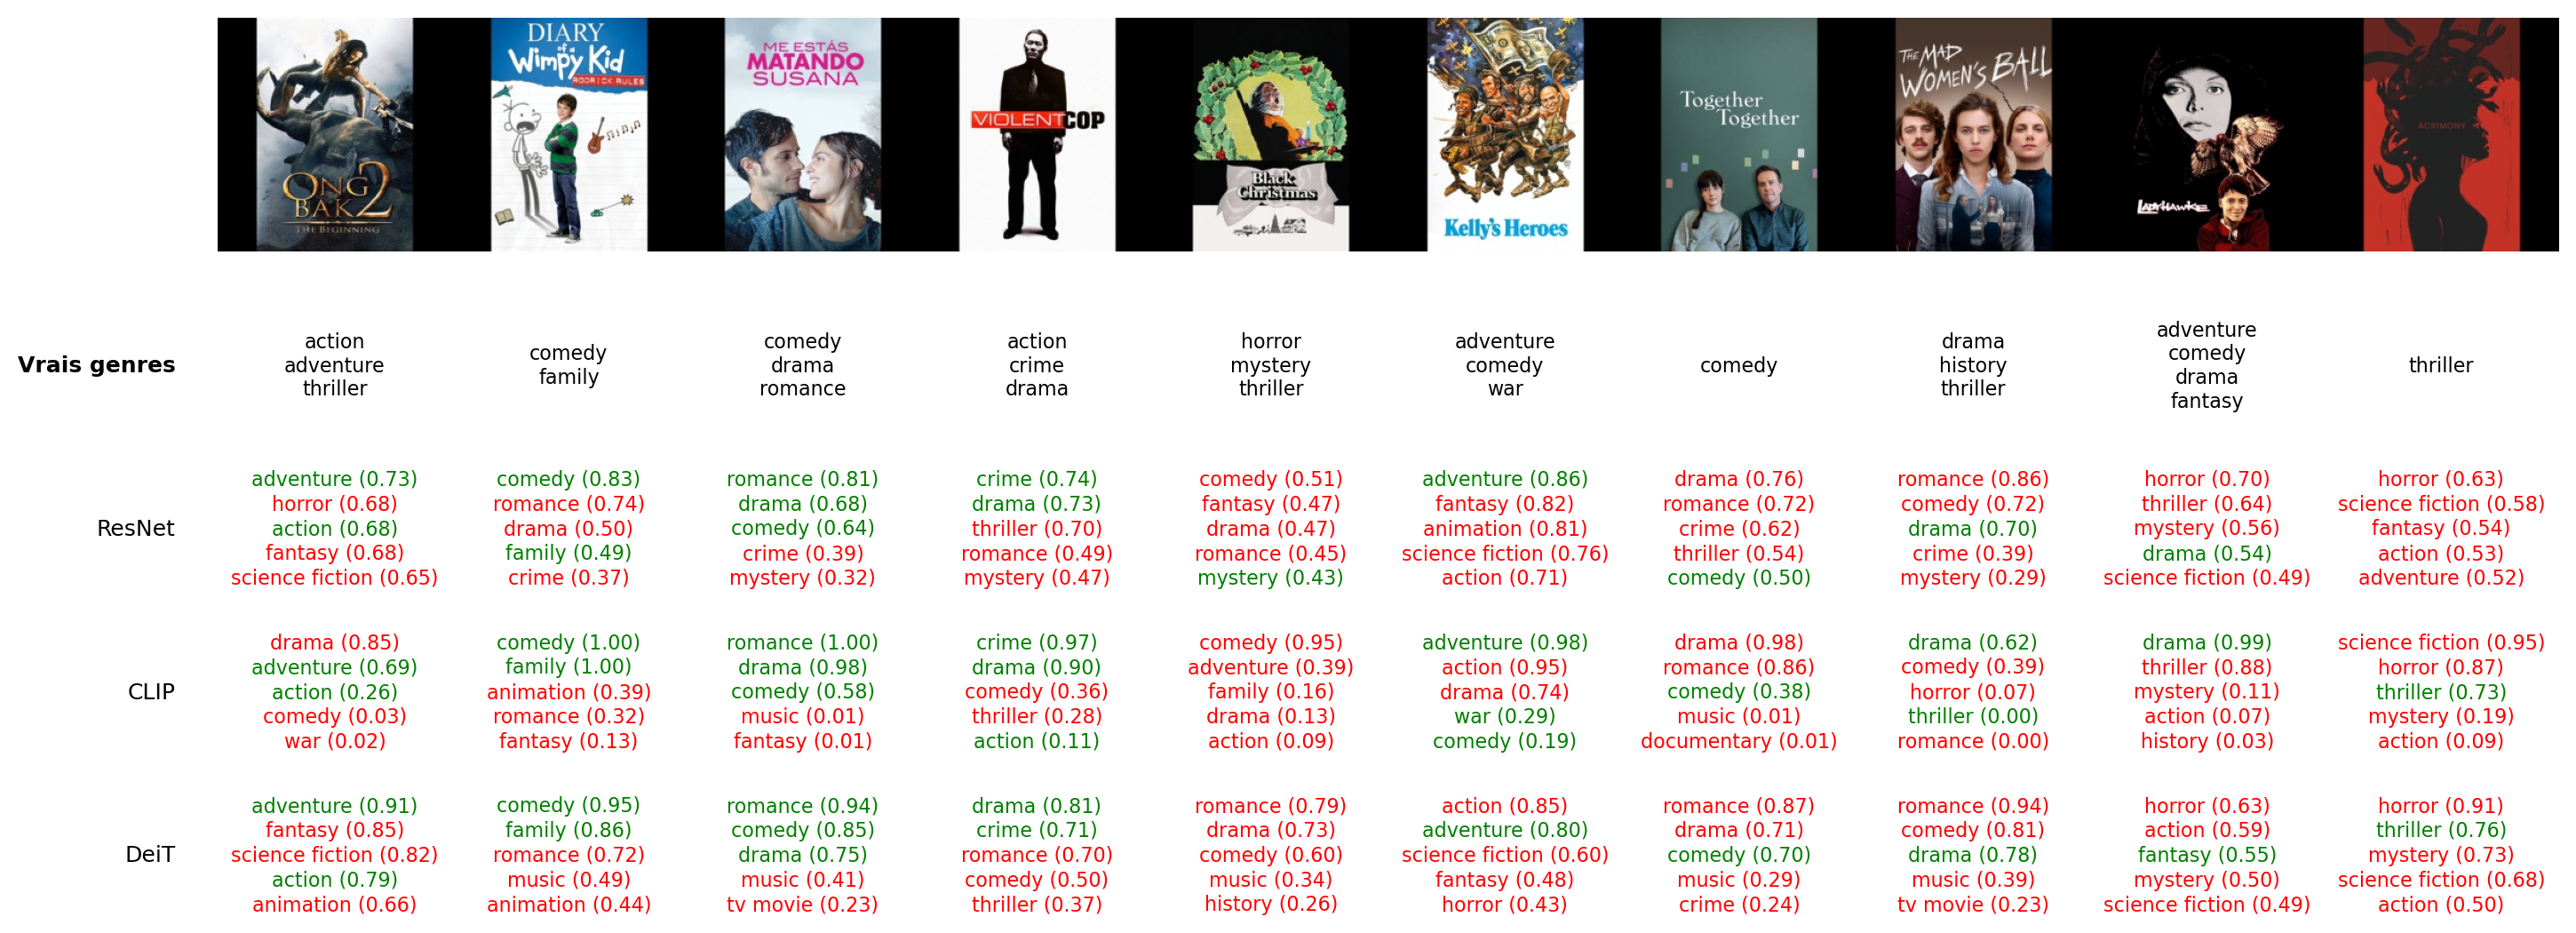
\includegraphics[width=\linewidth]{figures/test_predictions_grid.png}
\caption{Exemples qualitatifs de prédictions sur le jeu de test. La première ligne montre les posters, la seconde les vrais genres, et les lignes suivantes les $6$ genres les plus probables.}
\label{fig:prediction_test}
\end{figure}

La Figure~\ref{fig:prediction_test} illustre qualitativement le comportement des modèles. Les prédictions correctes montrent que les modèles capturent certains motifs visuels associés aux genres, par exemple les codes graphiques propres à l'action, à l'animation ou à l'horreur. Les erreurs restent cependant fréquentes lorsque les genres sont sémantiquement proches ou souvent co-occurrents, comme \emph{drama}, \emph{romance}, \emph{thriller} et \emph{crime}. Cette difficulté est naturelle dans un cadre multi-label : un même poster peut contenir des indices correspondant à plusieurs genres, et certains labels sont difficiles à distinguer à partir de l'image seule.

\section{Conclusion}

Nous avons comparé ResNet-50, DeiT-Small et CLIP ViT-B/32 pour la prédiction multi-label de genres à partir de posters.
CLIP fine-tuné obtient les meilleurs résultats, probablement grâce à son pré-entraînement image-texte.
Les limites principales viennent de l'ambiguïté des genres, de leurs co-occurrences et du déséquilibre du dataset.
Des pistes d'amélioration seraient l'utilisation de seuils spécifiques par genre, la calibration des probabilités ou l'agrégation de plusieurs modèles, ainsi que l'extraction explicite du texte présent sur les posters ou l'ajout de métadonnées comme le titre et le résumé du film.

{\footnotesize
\bibliographystyle{plain}
\bibliography{references}
}

\end{document}